\documentclass[11pt,a4paper]{article}
% Draft in a neutral single-column layout. To submit, paste the body into the official IJABC template
% (ABC 2027 site, "Template (IJABC)"); 8-12 pages including references.
\usepackage[margin=2.4cm]{geometry}
\usepackage[T1]{fontenc}
\usepackage{newtxtext,newtxmath}
\usepackage{graphicx}
\usepackage{booktabs}
\usepackage{multirow}
\usepackage{amsmath}
\usepackage{tikz}
\usetikzlibrary{arrows.meta,positioning,fit}
\usepackage[font=small,labelfont=bf]{caption}
\usepackage[hidelinks]{hyperref}
\usepackage{xcolor}

\title{Colour--Number Identities and Challenge-Style Re-Encoding\\for Player Tracking and Identification in 3x3 Basketball}
\author{Team \textsc{[name]} \\ \small [authors, affiliations, e-mail]}
\date{}

\begin{document}
\maketitle

\begin{abstract}
We describe our solution to the ABC 2027 TrackID3x3 Challenge: for every frame of a fixed-camera 3x3
basketball video, output the court position (in cm) and the identity (team and jersey number) of each
of the six players. TI-HOTA with $\tau = 100$\,cm evaluates the output, and a correct position with a wrong
identity scores nothing. Our pipeline has four steps:
\begin{enumerate}
\item A YOLO11l detector, fine-tuned in three rounds, finds the players, and BoT-SORT links the boxes over time.
\item A single ResNet18 classifier reads the bib colour and the jersey number of every box as one of
twelve (colour, number) identities plus ``other''. It can do this because each team wears the same
colour in every video.
\item The classifier probabilities are averaged along each tracklet. A per-frame Hungarian assignment
then gives each of the six roster identities at most one box.
\item The bottom-centre of each box is projected onto the court through the official homography.
Outliers are removed with a running median and with a physical speed limit, and gaps are interpolated.
\end{enumerate}
The Challenge videos differ from the Training videos in camera viewpoint, resolution, codec and dynamic
range. We therefore re-encode the Training videos to imitate the Challenge videos and use the
re-encoded frames both for training and for a realistic validation. On two held-out Training videos
processed this way, the final system reaches a TI-HOTA of 0.968, with a median position error of
5\,cm. We also report the changes that did not help, and an analysis of the metric: because the
evaluation compares exactly six predicted rows with six ground-truth rows per frame, TI-HOTA is
governed almost entirely by the localisation accuracy of correctly identified players.
\end{abstract}

\section{Introduction}
Tracking players and knowing who they are is the basis of most sports analytics: distances, speeds,
spacing, line-ups and tactical patterns all require trajectories attached to identities. The TrackID3x3
dataset~\cite{trackid3x3} provides 3x3 basketball videos with player boxes, court positions and
identities. The ABC 2027 TrackID3x3 Challenge asks for the complete chain, from video to court
trajectories of identified players.

Three properties of the Challenge shape our method.
\begin{itemize}
\item \textbf{Identity is part of the metric.} A predicted point counts only if both its team and its
jersey number are right. Jersey numbers also repeat across the two teams (e.g., both teams have a
number 6 and a number 9 in one Challenge game), so the team and the number must be recognised together.
\item \textbf{The ground truth is a projection of the box.} We found that the official court positions
are exactly the homography image of the bottom-centre of the annotated boxes. Position accuracy is
therefore box accuracy, measured at the feet.
\item \textbf{The Challenge videos are out of domain.} They come from a camera at a different position,
farther away and looking at the court at a flatter angle. They are also 720p, standard dynamic range and strongly compressed, whereas the Training videos
are 4K HDR.
\end{itemize}

Our contributions are:
\begin{enumerate}
\item \textbf{A joint colour--number identity classifier.} We observed that each of the four teams
wears a fixed bib colour throughout the dataset. Team assignment and jersey recognition therefore merge
into one 13-way classification of each box: twelve (colour, number) identities plus ``other''. The
classifier is trained only on the Training split.
\item \textbf{A Challenge-style re-encoding of the Training videos.} We map the Training videos from
HLG HDR to SDR, downscale them to 720p and encode them with H.264 at 3\,Mbit/s. The re-encoded videos
serve as training data for the detector and the classifier, and as a realistic validation set.
\item \textbf{Robust trajectory cleaning.} A running-median despike is combined with a segment filter
based on physical speed limits. The filter removes short wrong-player stretches and mid-air positions
during jump shots, an error that the oblique Challenge camera amplifies.
\item \textbf{A systematic evaluation.} We measure every design decision with TI-HOTA on held-out
videos, include the negative results, and analyse which errors the metric actually penalises.
\end{enumerate}

\section{Related Work}
\paragraph{Multi-object tracking in sports.}
Tracking-by-detection methods associate detector outputs over time. SORT~\cite{sort} and
DeepSORT~\cite{deepsort} combine a Kalman filter with motion and appearance cues. ByteTrack~\cite{bytetrack}
also uses low-confidence detections, and BoT-SORT~\cite{botsort} adds camera-motion compensation and
appearance (ReID) features. Sports scenes are harder than pedestrian scenes because players look alike,
move quickly and occlude each other often, as shown by SoccerNet-Tracking~\cite{soccernet} and
SportsMOT~\cite{sportsmot}. TrackID3x3~\cite{trackid3x3} adds identification and court localisation,
and introduces TI-HOTA, an identity-aware variant of HOTA~\cite{hota} in court coordinates. Its
baseline uses ID-switch merging and reaches a TI-HOTA of 85.5\% on the indoor subset and 71.0\% on the
outdoor subset (their Table~3, with $\tau = 1$\,m).

\paragraph{Player identification.}
Jersey numbers are usually read by dedicated digit recognisers or OCR~\cite{gerke}, and teams are
usually separated by clustering shirt colours. The Challenge tutorial baseline follows this pattern:
YOLO11x with ByteTrack, EasyOCR for numbers and HSV $k$-means for teams. Our setting allows a simpler and
more reliable formulation, because the bib colour of a team is constant and the roster of each game is
given. A single classifier then outputs the full identity, and the roster restricts it to six candidates.

\section{Data and Task Analysis}
\label{sec:data}
\paragraph{Training data.}
There are eight Training videos (IMG\_0104--0111) recorded with a fixed iPhone at 3840$\times$2160 and
30\,fps, about 6--7 minutes each. They total 93{,}581 frames and 561{,}256 annotated player boxes. For
every frame and each of the six players, the annotation gives a box, a court position in cm and an
identity. All videos share one court registration of four court corners. The players form four teams
that meet in different pairings. Table~\ref{tab:data} lists the properties that matter for our design.

\begin{table}[t]
\centering
\caption{Training and Challenge videos. The two splits differ in viewpoint, resolution, dynamic range and
compression.}
\label{tab:data}
\small
\resizebox{\linewidth}{!}{\begin{tabular}{lll}
\toprule
 & Training (8 videos) & Challenge (2 videos) \\
\midrule
Camera & fixed, elevated, diagonal view & fixed, other position, farther, flatter angle \\
Resolution & 3840$\times$2160, 30\,fps & 1280$\times$720, 30\,fps \\
Codec & HEVC Main10, HLG HDR (BT.2020), 29\,Mbit/s & H.264 Main, SDR (BT.709), 3\,Mbit/s \\
Frames & 10{,}706--13{,}228 per video & 11{,}536 and 11{,}823 \\
Player height (720p) & $\approx$\,85--150\,px (4K: 250--450\,px) & median $\approx$\,90\,px \\
Roster & tracks, teams, numbers, game start, offence & teams and numbers only \\
\bottomrule
\end{tabular}}
\end{table}

\paragraph{How the ground truth is built.}
We projected the bottom-centre of every annotated box with the homography estimated from the four
registered corners~\cite{hartley}. The result reproduces the official court positions to within
0.001\,cm on all videos that have them. The positions are therefore not measured separately: they inherit
any error of the box bottom. Two consequences follow:
\begin{itemize}
\item We must use the official registration file, even where the projected court lines visibly deviate
from the painted lines.
\item The detector must place the bottom edge of the box the way the annotators did. Detector
fine-tuning matters more than any change to the tracker.
\end{itemize}

\paragraph{Cleaning.}
We drop one off-roster box (a spectator in IMG\_0110). In IMG\_0105, 25 boxes are duplicated; for each
duplicate we keep the box whose foot point continues the track. We also read all videos sequentially:
seeking with OpenCV can be off by up to three frames on these files, and a one-frame offset already costs
0.01 TI-HOTA.

\paragraph{Fixed bib colours.}
We inspected all Training videos and found that each team always wears the same bib colour:
purple $\{4,10,12\}$, yellow $\{6,9,10\}$, green $\{6,9,11\}$ and pink $\{1,3,5\}$. The two Challenge
games also use these teams:
\begin{itemize}
\item IMG\_0114: A = yellow, B = green, with numbers 6 and 9 on both teams.
\item IMG\_0115: A = purple, B = pink.
\end{itemize}
Other people in the scene, such as substitutes, referees and spectators, wear other colours.

\paragraph{Split.}
We hold out IMG\_0108 and IMG\_0109, whose team pairings are the same as in the two Challenge games.
We train on the other six videos. The Challenge videos are used only for inference and for label-free
sanity checks, never for training, pseudo-labels or manual corrections.

\section{Method}
Figure~\ref{fig:pipeline} gives an overview of the pipeline.

\begin{figure}[t]
\centering
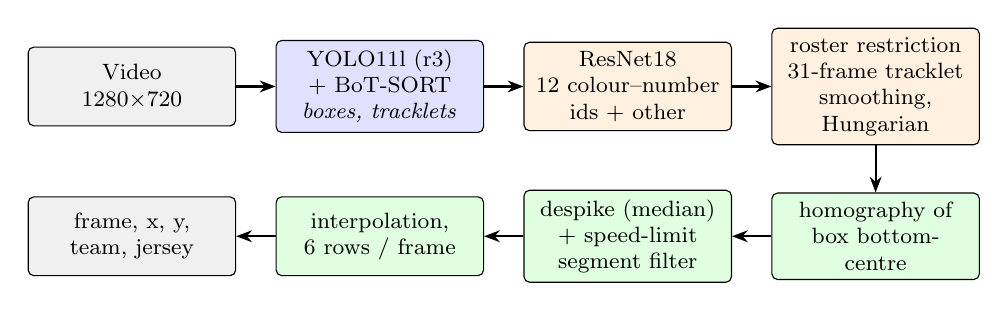
\begin{tikzpicture}[node distance=4mm and 5mm, every node/.style={font=\footnotesize},
  box/.style={draw, rounded corners=2pt, align=center, minimum height=10mm, fill=#1!12, text width=24mm},
  box/.default=gray, arr/.style={-{Stealth[length=2mm]}, thick}]
\node[box=gray] (v) {Video\\1280$\times$720};
\node[box=blue, right=of v] (d) {YOLO11l (r3)\\+ BoT-SORT\\\emph{boxes, tracklets}};
\node[box=orange, right=of d] (c) {ResNet18\\12 colour--number\\ids + other};
\node[box=orange, right=of c] (a) {roster restriction\\31-frame tracklet\\smoothing, Hungarian};
\node[box=green, below=6mm of a] (h) {homography of\\box bottom-centre};
\node[box=green, left=of h] (o) {despike (median)\\+ speed-limit\\segment filter};
\node[box=green, left=of o] (i) {interpolation,\\6 rows / frame};
\node[box=gray, left=of i] (out) {frame, x, y,\\team, jersey};
\draw[arr] (v) -- (d); \draw[arr] (d) -- (c); \draw[arr] (c) -- (a); \draw[arr] (a) -- (h);
\draw[arr] (h) -- (o); \draw[arr] (o) -- (i); \draw[arr] (i) -- (out);
\end{tikzpicture}
\caption{Overview. Blue: detection and tracking (Sec.~\ref{sec:det}). Orange: identification and
assignment (Sec.~\ref{sec:id}). Green: localisation and cleaning (Sec.~\ref{sec:loc}).}
\label{fig:pipeline}
\end{figure}

\subsection{Challenge-style re-encoding}
\label{sec:enc}
The Training videos are HLG-encoded HDR, whereas the Challenge videos are SDR exports. Simply
downscaling the Training frames therefore produces images with a different tone, saturation and noise
than the Challenge frames. We re-encode each Training video with FFmpeg in four steps:
\begin{enumerate}
\item Linearise the HLG signal (nominal peak 203\,cd/m$^2$).
\item Convert BT.2020 to BT.709 primaries and apply Hable tone mapping.
\item Downscale to 1280$\times$720 by area averaging.
\item Encode with H.264 Main at 2990\,kbit/s, matching the Challenge bit rate.
\end{enumerate}
We keep the frame timing unchanged, so every frame keeps its index and its labels; the 4K box
coordinates are simply divided by three. We use the re-encoded videos in three places: as extra
training images for the detector (round 3), as extra training crops for the identity classifier, and
as our main validation set.

\subsection{Detection and tracking}
\label{sec:det}
We fine-tune Ultralytics YOLO11l~\cite{yolo11}, initialised from COCO~\cite{coco}, as a one-class
player detector at an input size of 1280. The training images are every fifth frame of the six
training videos (14{,}149 images); validation uses every fifth frame of IMG\_0108/0109 (4{,}572 images).
Table~\ref{tab:rounds} summarises the three training rounds.
\begin{itemize}
\item \textbf{Round 1} uses every second training image, AdamW and a cosine schedule. Early stopping
selected epoch 2.
\item \textbf{Round 2} continues from round 1 on all images with SGD and lighter augmentation.
\item \textbf{Round 3} continues from round 2 on the Challenge-style frames. It adds rotation ($\pm5^\circ$),
shear ($\pm3^\circ$) and perspective augmentation to soften the change of viewpoint.
\end{itemize}
We select checkpoints by TI-HOTA of the full pipeline, not by detection mAP, for the reason given in
Sec.~\ref{sec:results}.

At inference we keep detections above confidence 0.1 and track them with BoT-SORT~\cite{botsort}. The
tracker settings are: high/low/new-track thresholds 0.25/0.1/0.25, a 90-frame buffer and match
threshold 0.8. We switch off camera-motion compensation because the camera is fixed, and we switch off
ReID (see Sec.~\ref{sec:neg}). The tracker only groups boxes into tracklets; identities come from the
next stage.

\begin{table}[t]
\centering
\caption{Detector fine-tuning rounds. The images are 720p frames from the six training videos. All rounds
use batch 5, image size 1280 and horizontal flips. mAP is measured on the validation frames of each round
(clean for r1/r2, Challenge-style for r3).}
\label{tab:rounds}
\small
\resizebox{\linewidth}{!}{\begin{tabular}{llllll}
\toprule
Round & Init & Images & Optimiser, epochs & Augmentation & mAP50 / 50--95 \\
\midrule
r1 & COCO YOLO11l & 7.1k clean & AdamW $2\!\cdot\!10^{-3}$, cos, 10 (best 2) & mosaic, scale 0.6 & 0.969 / 0.792 \\
r2 & r1 best & 14.1k clean & SGD $2\!\cdot\!10^{-3}$, 8 & mosaic 0.5, scale 0.3 & 0.995 / 0.668 \\
r3 & r2 last & 14.1k re-encoded & SGD $2\!\cdot\!10^{-3}$, 6 & + rot.\ 5$^\circ$, shear 3$^\circ$, persp. & 0.994 / 0.666 \\
\bottomrule
\end{tabular}}
\end{table}

\subsection{Identity classification and assignment}
\label{sec:id}
\paragraph{Classifier.}
Each box is enlarged by 10\% on every side and resized to 80$\times$160 pixels. A ResNet18~\cite{resnet}
initialised on ImageNet~\cite{imagenet} predicts 13 classes: the 12 (colour, number) identities and
``other''. Training crops come from the ground-truth boxes of the six training videos, cut from both the
clean frames and the Challenge-style frames.

To obtain ``other'' examples, we run a COCO person detector on the Training frames. Detections with
IoU < 0.1 to every player box become negatives (about 33k for training and 10k for validation).

The model is trained for 4{,}800 steps with batch 128, class-balanced sampling, label smoothing 0.05,
AdamW~\cite{adamw} at $10^{-3}$ and a one-cycle schedule. Augmentation simulates the Challenge view:
\begin{itemize}
\item box jitter and down/up-scaling to as little as 36\,px height;
\item rotation of $\pm6^\circ$;
\item brightness, saturation and gamma changes;
\item JPEG artefacts.
\end{itemize}
We use no horizontal flip, because it mirrors the digits, and no hue shift, because hue carries the team.
On Challenge-style validation crops, restricted to the six roster identities of each video (as the
pipeline uses them), the classifier is correct on 98.8\% of crops.

\paragraph{Assignment.}
For a video with roster identities $\mathcal{I} = \{1,\dots,6\}$, we keep the six corresponding
probabilities of every box and fold all others into ``other''. Single crops are noisy because of
occlusion, motion blur and turned backs, so we average the probability vectors along each tracklet with a
centred 31-frame moving window. Unlike a vote over the whole tracklet, a moving window follows an
identity switch inside a tracklet. In every frame $t$ we then solve
\begin{equation}
\max_{\pi} \sum_{(b,k) \in \pi} \bar{p}_{b,k}
\end{equation}
over one-to-one matchings $\pi$ between the boxes $b$ and the identities $k \in \mathcal{I}$, using the
Hungarian algorithm~\cite{kuhn}. A matched pair is kept only if $\bar{p}_{b,k} \geq 0.2$ and
$\bar{p}_{b,k} > 0.5\,\bar{p}_{b,\text{other}}$. The assignment guarantees at most one box per identity
per frame. Because it works per frame, a fragmented or switched tracklet costs only the frames in which
the classifier is wrong.

\subsection{Localisation, cleaning and interpolation}
\label{sec:loc}
The court position of an assigned box is the homography image of its bottom-centre (Sec.~\ref{sec:data}).
For each identity we then remove outliers in two steps.
\begin{enumerate}
\item \textbf{Despike.} A position is dropped if it lies more than 60\,cm from the median of the
identity's 15 neighbouring observations. This removes isolated wrong assignments.
\item \textbf{Segment filter.} The median cannot remove a wrong stretch that is as long as half its
window. We therefore cut the trajectory wherever consecutive observations at frames $f_i < f_j$ are
farther apart than $50 + 40\,(f_j - f_i)$\,cm, that is, faster than about 12\,m/s. A piece shorter than
30 observations is dropped if the pieces before and after it can be joined without it, or if it is at
an end of the trajectory next to a longer piece.
\end{enumerate}
The segment filter catches two kinds of error: a short assignment to the wrong player, and a jump shot.
During a jump the feet leave the floor, so the bottom of the box rises and projects metres away on an
oblique camera (Fig.~\ref{fig:jump}).

Finally, we fill the gaps by linear interpolation in time and hold the first and last positions
constant, so every frame $1..N$ has exactly six rows. The ground truth also has six rows per frame,
including the frames before the game starts.

\begin{figure}[t]
\centering
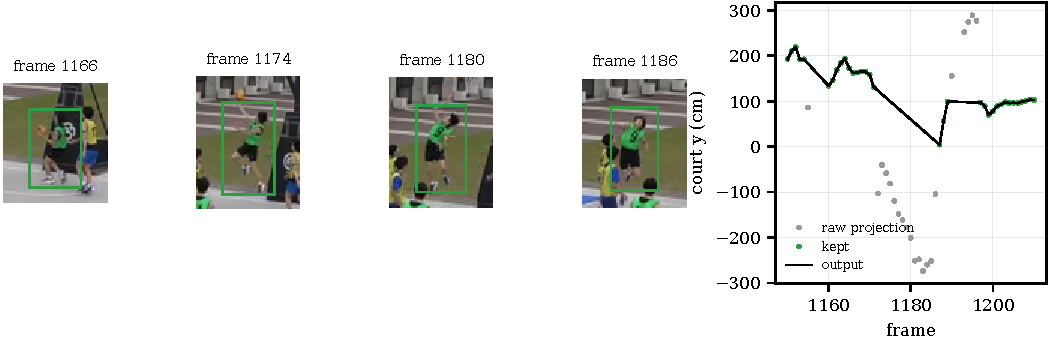
\includegraphics[width=\linewidth]{figures/jump.pdf}
\caption{A jump shot in Challenge video IMG\_0114 (player B9). Left: the feet leave the floor and the box
bottom rises. Right: the raw projected court $y$ jumps by more than a metre. The segment filter drops the
airborne stretch (grey), and the output (black) interpolates between take-off and landing.}
\label{fig:jump}
\end{figure}

\section{Experiments}
\label{sec:results}
\paragraph{Protocol.}
We report TI-HOTA with $\tau = 100$\,cm and use our own re-implementation, which we checked line by line
against the organisers' notebook. For each frame the metric computes the similarity
$s = \exp\!\big(\ln(0.05)\, d^2/\tau^2\big)$ for each ground-truth/prediction pair with the same identity,
and $s = 0$ otherwise. It then solves a Hungarian matching and computes $\sqrt{\text{DetA} \cdot \text{AssA}}$
at each threshold $\alpha \in \{0.05, \dots, 0.95\}$, and averages over $\alpha$. At $\alpha = 0.95$, a
match must lie within 13\,cm.

We score the mean over IMG\_0108 and IMG\_0109 in two versions: \emph{clean}, the 4K frames downscaled
to 720p, and \emph{Challenge-style}, the re-encoded videos of Sec.~\ref{sec:enc}. The Challenge-style
version is our main criterion.

\paragraph{What TI-HOTA rewards.}
Both the ground truth and our output contain exactly six rows per frame. Hence at every $\alpha$ we have
FP = FN = $6N - \text{TP}$. If $q_\alpha$ is the fraction of rows matched at threshold $\alpha$, then
\begin{equation}
\text{DetA}_\alpha = \frac{q_\alpha}{2 - q_\alpha}.
\end{equation}
With correct identities, AssA$_\alpha \approx$ DetA$_\alpha$. Averaging over $\alpha$ gives
$\text{TI-HOTA} \approx p/(2-p)$, where $p$ is the mean similarity per row. A loss of 1\% in $p$ therefore
costs about 2\% in TI-HOTA.

Two consequences shape our design:
\begin{itemize}
\item Emitting a guessed (interpolated) position is never worse than emitting nothing, so we always output
six rows.
\item A wrong identity scores zero, whatever its position.
\end{itemize}
We measured the metric's sensitivity directly. Random position noise of about 13\,cm gives 0.95, and noise
of about 50\,cm gives 0.46. Shifting all frame indices by one frame costs 0.01, and by three frames costs 0.11.

\begin{table}[t]
\centering
\caption{Development of the pipeline: TI-HOTA, mean of IMG\_0108/0109 (never used for training). Every
row adds one change to the row above. ``--'' = not run in that version.}
\label{tab:main}
\small
\begin{tabular}{lcc}
\toprule
Configuration & Clean & Challenge-style \\
\midrule
COCO YOLO11l + ByteTrack, identity by whole-tracklet vote (IMG\_0108 only) & 0.663 & -- \\
\;+ 31-frame smoothing and per-frame Hungarian assignment & 0.887 & -- \\
\;+ fine-tuned detector r1, best checkpoint (epoch 2) & 0.932 & -- \\
\;\;\; r1, last checkpoint (epoch 10) & 0.962 & -- \\
\;+ despike (60\,cm from 15-point median) & 0.963 & -- \\
\;+ detector r2 & 0.967 & 0.962 \\
\;+ classifier trained with Challenge-style crops & 0.966 & 0.962 \\
\;+ BoT-SORT instead of ByteTrack & -- & 0.962 \\
\;+ detector r3 (Challenge-style frames, geometric augmentation) & -- & \textbf{0.968} \\
\;+ segment filter (final) & -- & \textbf{0.968} \\
\bottomrule
\end{tabular}
\end{table}

\paragraph{Main results.}
Table~\ref{tab:main} traces the pipeline from a COCO detector to the final system.
\begin{itemize}
\item \textbf{Identity assignment matters most early on.} Replacing a whole-tracklet vote with a
smoothed per-frame assignment adds 0.22, because one wrong identity on a long tracklet otherwise
removes the whole trajectory.
\item \textbf{Detector fine-tuning brings the next largest gain.} It makes the boxes tight at the feet.
\item \textbf{Mild compression costs little.} The Challenge-style re-encoding lowers the score by only
0.005, so compression and tone mapping are not the main risk.
\item \textbf{Round 3 adds 0.006 on the Challenge-style videos,} and improves both videos (IMG\_0108
0.964 $\rightarrow$ 0.969, IMG\_0109 0.960 $\rightarrow$ 0.967).
\item \textbf{The segment filter leaves the validation score unchanged,} because the held-out videos
contain no stretch it removes. On the Challenge videos it removes exactly two stretches, and on
inspection both are errors: a wrong-player stretch and a jump shot (Fig.~\ref{fig:jump}).
\end{itemize}

\paragraph{Detection mAP does not predict TI-HOTA.}
The best round-1 checkpoint by mAP50--95 (0.792) scores 0.932 TI-HOTA. The last round-1 checkpoint has a
lower mAP50--95 (0.726) but scores 0.962. Later rounds lower mAP50--95 further while raising TI-HOTA.
The annotated boxes appear to be precise at the feet, which is what TI-HOTA measures, but looser at the
head and arms, which mAP50--95 also weighs. For this reason we select checkpoints only by TI-HOTA of the
full pipeline.

\paragraph{Where the remaining error is.}
With the final system, the median position error is 4--5\,cm for every player on both videos.
Table~\ref{tab:err} splits the rows by error:
\begin{itemize}
\item 93\% of rows are within 15\,cm. They earn almost the full score.
\item 6\% of rows are between 15 and 50\,cm. They cause most of the lost similarity, mainly during
occlusions, when the visible box bottom is not the feet.
\item Less than 1\% of rows are off by more than 50\,cm.
\item No row is missing or assigned to the wrong player.
\end{itemize}
Identification is therefore essentially solved on the held-out videos, and the remaining gap is
localisation under occlusion.

\begin{table}[t]
\centering
\caption{Error breakdown of the final system on the Challenge-style validation videos: share of rows and of
the similarity lost, per distance band.}
\label{tab:err}
\small
\resizebox{\linewidth}{!}{\begin{tabular}{lcccc|c}
\toprule
 & $<$15\,cm & 15--50\,cm & 50--200\,cm & $>$200\,cm / wrong id & mean similarity $p$ \\
\midrule
IMG\_0108 rows (lost) & 93.1\% (0.001) & 6.1\% (0.009) & 0.8\% (0.006) & 0.0\% (0.000) & 0.984 \\
IMG\_0109 rows (lost) & 92.7\% (0.001) & 6.4\% (0.010) & 0.9\% (0.007) & 0.0\% (0.000) & 0.983 \\
\bottomrule
\end{tabular}}
\end{table}

\subsection{What did not help}
\label{sec:neg}
Table~\ref{tab:neg} lists the variants we rejected. We report them because several of them would be
reasonable defaults in other tracking problems.
\begin{itemize}
\item \textbf{Test-time augmentation.} Flips and multiple scales blur the bottom edge of the box, and
the share of rows in the 15--50\,cm band grows from 7\% to 10--12\%.
\item \textbf{BoT-SORT with ReID.} It is 2.5$\times$ slower and slightly worse. Identities come from the
classifier, so better tracklet appearance matching has little to add.
\item \textbf{Interpolating over occlusions.} The detector's estimate of an occluded player's feet is
still better than interpolating over the occlusion.
\item \textbf{Temporal smoothing of positions.} It lowered TI-HOTA, because any lag costs points at the
strict thresholds.
\item \textbf{A longer segment window.} Raising the minimum piece length from 30 to 60 starts removing
correct stretches.
\end{itemize}

\begin{table}[t]
\centering
\caption{Rejected variants (TI-HOTA, IMG\_0108/0109; the reference uses the same validation version).}
\label{tab:neg}
\small
\begin{tabular}{lcc}
\toprule
Variant & Score & Reference \\
\midrule
Test-time augmentation (flip + scales) & 0.956 & 0.962 \\
BoT-SORT with ReID features & 0.960 & 0.962 \\
Replace occluded positions by interpolation (clean) & 0.917--0.962 & 0.963 \\
Segment filter with minimum length 60 & 0.9675 & 0.9680 \\
Detector r3 after 1 / 3 of 6 epochs & 0.953 / 0.966 & 0.968 \\
\bottomrule
\end{tabular}
\end{table}

\subsection{The Challenge videos}
We have no labels for the Challenge videos, so we checked the outputs in label-free ways.

\paragraph{Basic checks.} We verified that:
\begin{itemize}
\item the official court registration aligns with the painted court lines;
\item every frame has the six roster identities;
\item drawn frames show the expected bib colours for teams A and B (Fig.~\ref{fig:views});
\item the trajectories look plausible (Fig.~\ref{fig:court}).
\end{itemize}

\paragraph{Unsupervised statistics can mislead.}
We also tracked unsupervised statistics: the number of player tracklets, the share of uncertain crops,
and the number of jumps above 1\,m per frame. They are useful to spot gross failures, but they did not
rank models correctly. With the round-3 detector, the Challenge outputs show more uncertain crops
(IMG\_0114: 21\% $\rightarrow$ 28\%) and more jumps above 1\,m (6 $\rightarrow$ 12) than with round 2.
Yet the same shift on the held-out videos (uncertain crops 2.5\% $\rightarrow$ 6.5\%, jumps
3 $\rightarrow$ 6 on IMG\_0108) came with a higher TI-HOTA. The new detector simply finds more people,
including bystanders, and the classifier rejects them as ``other''. The round-2 and round-3 Challenge
outputs agree within 30\,cm on 96\% of rows, with a median difference of 8--9\,cm.

\begin{figure}[t]
\centering
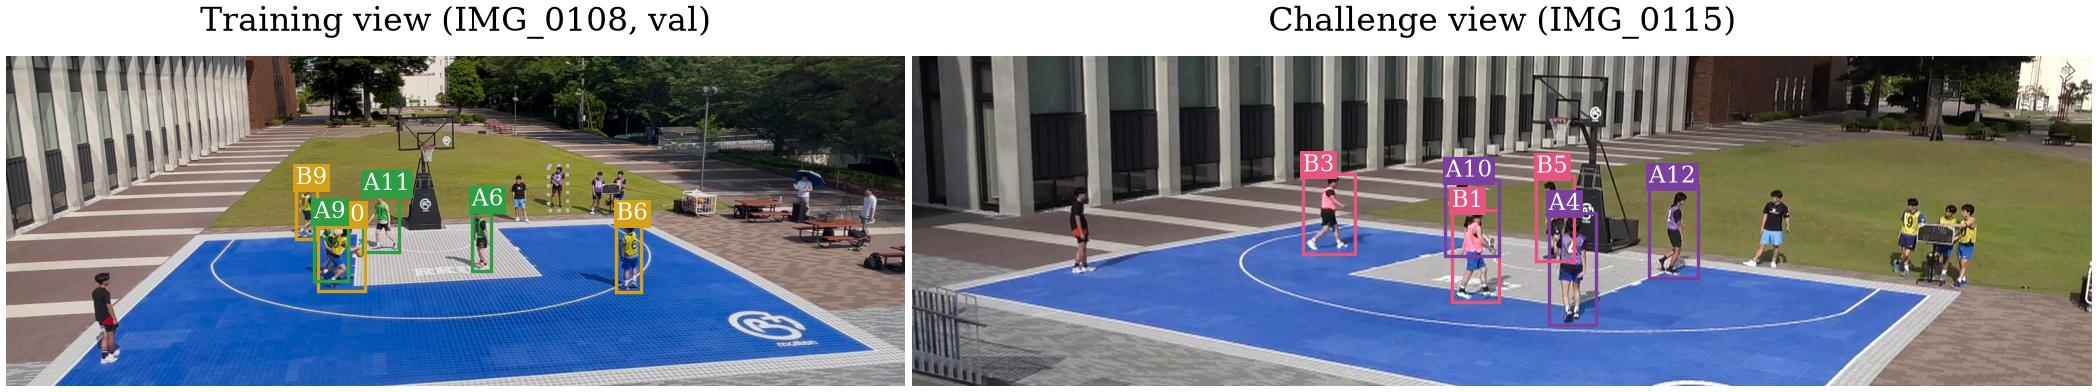
\includegraphics[width=\linewidth]{figures/views.jpg}
\caption{Training view (left, held-out IMG\_0108 after Challenge-style re-encoding) and Challenge view
(right, IMG\_0115), with the identities assigned by our pipeline. Dotted grey boxes are detections
classified as ``other''.}
\label{fig:views}
\end{figure}

\begin{figure}[t]
\centering
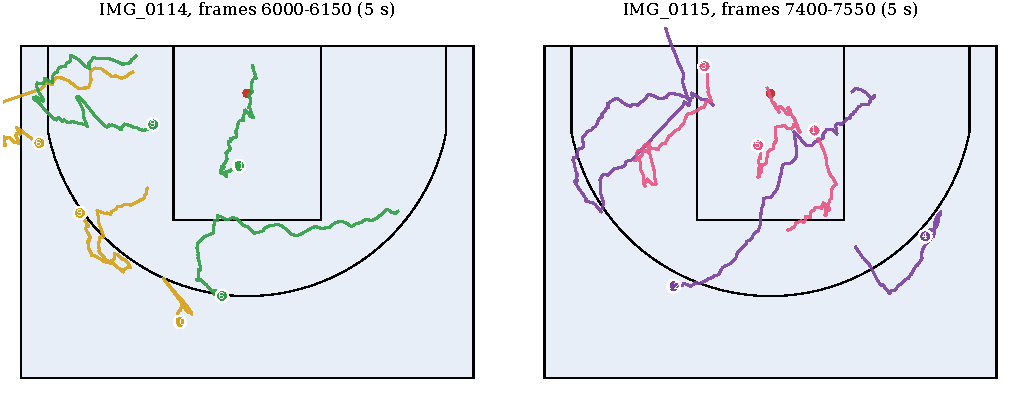
\includegraphics[width=\linewidth]{figures/court.pdf}
\caption{Five seconds of predicted trajectories on the two Challenge videos, coloured by bib colour; the dot
marks the last position, labelled with the jersey number. The jitter of a few tens of centimetres comes from
frame-to-frame variation of the box bottom; we do not smooth positions (Sec.~\ref{sec:neg}).}
\label{fig:court}
\end{figure}

\section{Discussion and Limitations}
\begin{itemize}
\item \textbf{Viewpoint.} The change of viewpoint is the risk we cannot measure: the held-out videos
share the Training camera. We softened it with geometric augmentation and Challenge-style frames, and
with a classifier that sees players from several angles within the Training videos. The flatter
viewing angle of the Challenge camera also changes the geometry of the error. A given vertical offset of the box
bottom, from a jump or an occlusion, maps to a larger court distance than in the Training view, so we
expect the Challenge score to be lower than on validation.
\item \textbf{Optimistic validation.} We chose all hyper-parameters (the 31-frame window, the 60\,cm
despike threshold, the checkpoints) on IMG\_0108/0109, so the validation numbers are somewhat optimistic.
\item \textbf{Fixed bib colours.} The joint colour--number formulation relies on fixed team colours. It
transfers to leagues with fixed kits, but a new team requires new training crops. Separate colour and
number heads would generalise better.
\item \textbf{Future work.} Most of the remaining error comes from occlusion. Modelling the feet
explicitly, for example with pose keypoints or a learned foot point, could reduce it.
\end{itemize}

\section{Conclusion}
We presented a tracking-and-identification pipeline for 3x3 basketball built around three observations.
The court positions are projected box bottoms. Teams wear fixed bib colours, so identity is a 13-way
classification. The Challenge videos differ from the Training videos in encoding as well as viewpoint.
A fine-tuned YOLO11l detector, a joint colour--number classifier with per-frame Hungarian assignment,
and speed-limit trajectory cleaning reach a TI-HOTA of 0.968 on held-out videos re-encoded like the
Challenge videos. Every component was trained on the official Training split only. The code, weights and
a one-command script that reproduces the submitted predictions accompany this paper.

\begin{thebibliography}{99}\small
\bibitem{trackid3x3} K.~Yamada, L.~Yin, Q.~Hu, N.~Ding, S.~Iwashita, J.~Ichikawa, K.~Kotani, C.~Yeung, K.~Fujii.
TrackID3x3: A dataset and algorithm for multi-player tracking with identification and pose estimation in 3x3
basketball full-court videos. In \emph{Proc.\ 8th ACM Int.\ Workshop on Multimedia Content Analysis in Sports
(MMSports)}, pp.~163--173, 2025.
\bibitem{hota} J.~Luiten, A.~O\v{s}ep, P.~Dendorfer, P.~Torr, A.~Geiger, L.~Leal-Taix\'e, B.~Leibe.
HOTA: A higher order metric for evaluating multi-object tracking. \emph{Int.\ J.\ Computer Vision}, 129(2):548--578, 2021.
\bibitem{sort} A.~Bewley, Z.~Ge, L.~Ott, F.~Ramos, B.~Upcroft. Simple online and realtime tracking. In \emph{ICIP}, 2016.
\bibitem{deepsort} N.~Wojke, A.~Bewley, D.~Paulus. Simple online and realtime tracking with a deep association metric. In \emph{ICIP}, 2017.
\bibitem{bytetrack} Y.~Zhang, P.~Sun, Y.~Jiang, D.~Yu, F.~Weng, Z.~Yuan, P.~Luo, W.~Liu, X.~Wang.
ByteTrack: Multi-object tracking by associating every detection box. In \emph{ECCV}, 2022.
\bibitem{botsort} N.~Aharon, R.~Orfaig, B.-Z.~Bobrovsky. BoT-SORT: Robust associations multi-pedestrian tracking.
arXiv:2206.14651, 2022.
\bibitem{soccernet} A.~Cioppa, S.~Giancola, A.~Deli\`ege, et al. SoccerNet-Tracking: Multiple object tracking dataset and
benchmark in soccer videos. In \emph{CVPR Workshops}, 2022.
\bibitem{sportsmot} Y.~Cui, C.~Zeng, X.~Zhao, Y.~Yang, G.~Wu, L.~Wang. SportsMOT: A large multi-object tracking dataset in
multiple sports scenes. In \emph{ICCV}, 2023.
\bibitem{gerke} S.~Gerke, K.~M\"uller, R.~Sch\"afer. Soccer jersey number recognition using convolutional neural networks.
In \emph{ICCV Workshops}, 2015.
\bibitem{yolo11} G.~Jocher, J.~Qiu. Ultralytics YOLO11. \url{https://github.com/ultralytics/ultralytics}, 2024.
\bibitem{coco} T.-Y.~Lin, M.~Maire, S.~Belongie, et al. Microsoft COCO: Common objects in context. In \emph{ECCV}, 2014.
\bibitem{resnet} K.~He, X.~Zhang, S.~Ren, J.~Sun. Deep residual learning for image recognition. In \emph{CVPR}, 2016.
\bibitem{imagenet} J.~Deng, W.~Dong, R.~Socher, L.-J.~Li, K.~Li, L.~Fei-Fei. ImageNet: A large-scale hierarchical image
database. In \emph{CVPR}, 2009.
\bibitem{adamw} I.~Loshchilov, F.~Hutter. Decoupled weight decay regularization. In \emph{ICLR}, 2019.
\bibitem{kuhn} H.~W.~Kuhn. The Hungarian method for the assignment problem. \emph{Naval Research Logistics Quarterly},
2(1--2):83--97, 1955.
\bibitem{hartley} R.~Hartley, A.~Zisserman. \emph{Multiple View Geometry in Computer Vision}, 2nd ed. Cambridge
University Press, 2004.
\end{thebibliography}

\end{document}
